% !TEX TS-program = pdflatex
% !TEX encoding = UTF-8 Unicode

% This is a simple template for a LaTeX document using the "article" class.
% See "book", "report", "letter" for other types of document.

\documentclass[10pt]{article} % use larger type; default would be 10pt
\usepackage[utf8]{inputenc} % set input encoding (not needed with XeLaTeX)
\usepackage{framed}
\usepackage[utf8]{inputenc}
\usepackage[T1]{fontenc}
\usepackage{csquotes}
\usepackage{booktabs}
\usepackage{wrapfig}
\usepackage[english]{babel}
\usepackage{blindtext}
\usepackage{lettrine}
%%% Examples of Article customizations
% These packages are optional, depending whether you want the features they provide.
% See the LaTeX Companion or other references for full information.

%%% PAGE DIMENSIONS
\usepackage{geometry} % to change the page dimensions
\setlength{\abovecaptionskip}{10pt plus 5pt minus 3pt}
\usepackage{wrapfig}
\geometry{a4paper} % or letterpaper (US) or a5paper or....
% \geometry{margin=2in} % for example, change the margins to 2 inches all round
% \geometry{landscape} % set up the page for landscape
%   read geometry.pdf for detailed page layout information

\usepackage{graphicx} % support the \includegraphics command and options
\usepackage{amsthm, amsmath, wasysym, MnSymbol}
\usepackage{booktabs} % Top and bottom rules for table
\usepackage[font=small,labelfont=bf]{caption} % Required for specifying captions to tables and figures
% \usepackage[parfill]{parskip} % Activate to begin paragraphs with an empty line rather than an indent

%%% PACKAGES

\usepackage{booktabs} % for much better looking tables
\usepackage{array} % for better arrays (eg matrices) in maths
\usepackage{paralist} % very flexible & customisable lists (eg. enumerate/itemize, etc.)
\usepackage{verbatim} % adds environment for commenting out blocks of text & for better verbatim
\usepackage{subfig} % make it possible to include more than one captioned figure/table in a single float
% These packages are all incorporated in the memoir class to one degree or another...

%%% HEADERS & FOOTERS
\usepackage{fancyhdr} % This should be set AFTER setting up the page geometry
\pagestyle{fancy} % options: empty , plain , fancy
\renewcommand{\headrulewidth}{0pt} % customise the layout...
\lhead{}\chead{}\rhead{}
\lfoot{}\cfoot{\thepage}\rfoot{}
%%% SECTION TITLE APPEARANCE
\usepackage{sectsty}
\allsectionsfont{\sffamily\mdseries\upshape} % (See the fntguide.pdf for font help)
% (This matches ConTeXt defaults)

%%% ToC (table of contents) APPEARANCE
\usepackage[nottoc,notlof,notlot]{tocbibind} % Put the bibliography in the ToC
\usepackage[titles,subfigure]{tocloft} % Alter the style of the Table of Contents
\renewcommand{\cftsecfont}{\rmfamily\mdseries\upshape}
\renewcommand{\cftsecpagefont}{\rmfamily\mdseries\upshape} % No bold!

%%% END Article customizations

%%% The "real" document content comes below...
\font\loll= cmr25 at 45pt
\title{ \loll Thermal analysis on a turbulent Poiseuille flow}
\author{Aristeu da Silveira Neto,  Felipe J. O. Ribeiro.}
%\date{} % Activate to display a given date or no date (if empty),
         % otherwise the current date is printed 

\begin{document}
\maketitle

\begin{figure}[h!]
	\centering
	
\includegraphics[angle=0, scale=0.60]{turbulence}
	\label{turbulence}
\end{figure}

\begin{abstract}
	\noindent Fluid dynamics is a subject of great academic and industrial interest. It offers many opportunities for optimization in a variety of practical engineering problems. The modeling of thermal properties of turbulent flows is something of remarkable complexity, that can be explained mathematically by the chaotic nature of this non-linear high order differential analysis, fact beautifully stated in the Strogatz`s book "Nonlinear Dynamics and Chaos". The immediate result of such fact is the impossibility of an exact mathematical answer for, near, all real applications. The only way of gathering results, then, is by an numerical approach, with the discretization of space and time, for an approximate result. The problem is that, in most cases, these are a so big computational problem that become inviable as the mathematical differential methodology require a big number of computers for a big amount of time. With that in mind, the present paper aims to develop a semi-exact meta-modeled approach on a turbulent Poiseuille flow thermal analysis over a channel, aiming on efficiency and accuracy when compared to the DNS solution, the most respected but computational expensive method there is. 
\end{abstract}




\pagebreak

\begin{LARGE}
	Nomenclature: 
\end{LARGE} 


	Pr = Molecular Prandtl number.
	
	
	
	
	$Re$ = Reynolds number. $Re = \frac{2R \overline{U}}{\nu}$
	
	
	$Re_\tau$ = Turbulent Reynolds number. $Re_\tau = \frac{R U_\tau}{\nu}$
	
	
	
	T = temperature.
	
	
	${\overline{T}}$ = Temperature mean value.
	
	
	
	$T_\tau$ = Friction temperature. $\frac{q_w}{\rho c_p u_\tau}$ 
	
	
	
	
	$\overline{U}_c$ = Mean velocity on channel`s center.
	
	
	
	u , v , w = velocities components on each axis.
	
	
	$u^\prime $ , $ v^\prime $ , $ w^\prime $ = Fluctuations of velocity on each axis.
	
	
	$U_\tau$ = Friction velocity.
	
	
	x , y , z = Cartesian classic coordinates.
	
	
	$\tilde{y} $= $ y \frac{u_\tau}{R} $
	
	
	R = Mean channel length.
	
	
	
	$\nu$ = kinetic viscosity.
	
	
	$\nu_\tau$ = Turbulent viscosity.
	
	
	$\rho$ = Density.
	
	
	$\alpha$ = Thermal diffusivity.
	
	
	$\alpha_t$ = Turbulent thermal diffusivity. 
	
	
	$\tilde{()}$ = Normalized under wall properties.
	
	$\overline{()}$ = mean value.  



\tableofcontents

\section{Introduction}

\lettrine[nindent=0em,lines=2]{I}s well known that the field of turbulent diffusion is of such hight complexity that, even nowadays, it is not completely understood, as described by O. Basim and Hasan, 2007 \cite{hasan}. Out of the domain of Direct Numerical Solutions (DNS), all sorts of experimental approximations have to be assumed to properly mathematically develop the Navier-Stokes equations as the nonlinear behavior of these systems \cite{John} make difficult for an exact mathematical solution.  For that, in this work, the mixing length model was used, by Ludwig Prandtl, that rely on the Boussinesq hypothesis for being a way of modeling the Reynolds tensor on the development of the Navier-Stokes equation.\\ 
On this context, some parameters that worth mentioning are the turbulent Prandtl number \cite{Prandtl} and the constant $A = 26$, on Cebeci`s damping formulation \cite{Cebeci} (Eq. \ref{cebeci}):

\begin{equation}\label{cebeci}
\frac{l_m}{R} = \left( 0.14 - 0.08 \left(\frac{y}{R}\right)^2 - 0.06\left(\frac{y}{R}\right)^4\right) \\
\left\{  1 - e^{[(\tilde{y} - 1) \frac{Re_\tau}{A}]}\right\}.	
\end{equation}

These physical terms are responsible for modeling important properties of the fluid`s thermal diffusion and dynamics as said by S. N. Aristeu, 2018 \cite{aristeu}. Such parameters models are examples of approximations that are necessary to implement a semi analytical method, like RANS, URANS and LES \cite{aristeu}. It consists in not numerically resolving the Naiver-Stokes equation on all scales required, but instead substituting some tensors and other nonlinear therms by conceptual and experimental approximations.

Such methods are important because they offer a much quicker solution. The DNS approach demands high computational work, not even being possible or viable in some cases, as explained on H. Kawamura, H. Abe and Yuichi Matsuo's work \cite{Abe}. An example of this is for high Reynolds number systems. But, in other hand, these approximated methods result in some errors in comparison with the DNS solution.    

On the present paper, the authors aim to develop a semi analytical RANS (Reynold`s Averaged Navier-Stokes) method to describe the thermal configuration on a turbulent plane Poiseuille flow \cite{Poiseuille}, modeled with the mixture length methodology. Meta-models were developed defining the turbulent Prandtl number \cite{Prandtl} and the constant $A = 26$, on Cebeci`s damping formulation, to enhance the results compared to DNS solutions, resulting on accuracy and efficiency. The results of this work's formulation were compared with the DNS available (\cite{DNS1020} , \cite{DNS150}), aiming to provide an analysis on the viability of meta models on turbulent Poiseuille flows thermal problems.\\       
 

\section{Physical model}

The problem was defined as a plane channel flow, with only one finite dimension on the $y$ axis. Two boundary walls were set as two nonslip infinite plates in a constant heat regime. The $z$ axis was proposed self similar both on velocity and temperature, resulting on a plane domain (Fig.\ref{figure.1}). \\
The fluid was incompressible and Newtonian. It was flowing on the $x$ axis direction on Reynolds numbers that variated from $4560$ to $41441$, resulting on a turbulent regime domain. 

\begin{figure}[h!]
	\centering
	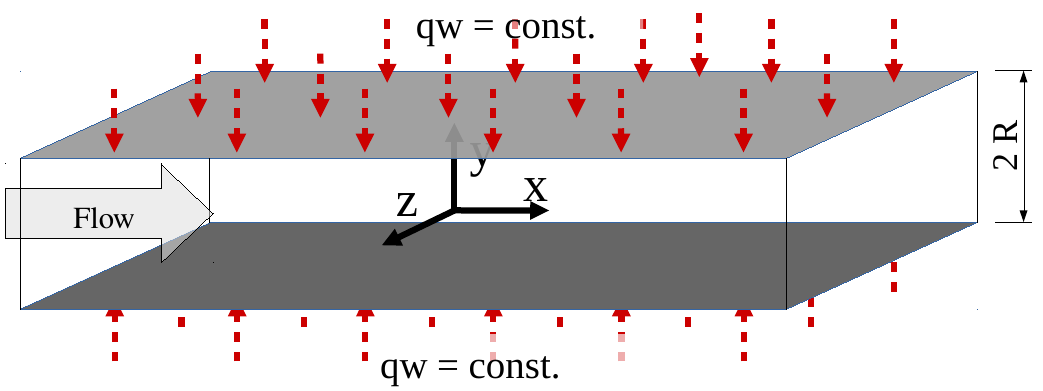
\includegraphics[angle=0, scale=0.50]{figure1}
	\caption{Geometric definition and boundary condition of the system.}
	\label{figure.1}
\end{figure}

The base mathematical formulation for the problem where the continuity and Navier-Stokes equations as defined on Cengel's book \cite{Cengel}, and the  energy transport equation, as defined on Freank's Incropera \cite{Incropera}. These were the assumptions made to the proposed problem, that will be considered on the mathematical model ahead.









\section{Differential model}

Developing the thermal energy equation, the continuity equation and the Navier-Stokes equations for mean statistical permanent regimes resulted on: 


\begin{equation}\label{energy permanent}
\frac{\partial{}}{\partial{x}} \left(\overline{T^\prime u^\prime}\right) + \frac{\partial{}}{\partial{x}}\left(\overline{u}.\overline{T}\right)     + 
\frac{\partial{}}{\partial{y}} \left(\overline{T^\prime v^\prime}\right) + \frac{\partial{}}{\partial{y}}\left(\overline{v}.\overline{T}\right) 
=
{\frac{\partial{}}{\partial{x}}} \left(\alpha {\frac{\partial{\overline{T}}}{\partial{x}}} \right) +
{\frac{\partial{}}{\partial{y}}} \left(\alpha {\frac{\partial{\overline{T}}}{\partial{y}}} \right). 
\end{equation}

\begin{equation}\label{mass}
\frac{\partial \overline{u}}{\partial x} = 0.
\end{equation}

\begin{equation}\label{dynamics}
\frac{\partial \overline{u}\overline{v}}{\partial y} = 
- \frac{1}{\rho} \frac{\partial \overline{p}}{\partial x} + \frac{\partial}{\partial y}\left(\nu \frac{\partial \overline{u}}{\partial y} - \overline{u^\prime v^\prime}\right).
\end{equation}

Where (\ref{energy permanent}) represents the mean energy balance for a given point, the (\ref{mass}) represents the mean mass balance and (\ref{dynamics}) represents de mean linaer momentum balance. All of these beeing for the same given point.

\subsection{The temperature permanent regime}

Even when on simplified mean values, the temperature field of a turbulent channel flow don't converge naturally to a unidimensional permanent state (fig.\ref{figure.2}).

\begin{figure}[h!]
	\centering
	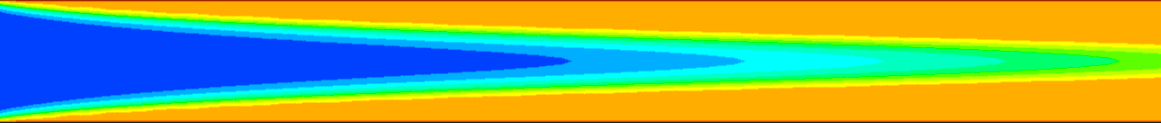
\includegraphics[angle=0, scale=0.40]{temperatura}
	\caption{Temperature field in statistical permanent regime over a channel.}
	\label{figure.2}
\end{figure}
 
 To make this happen, the boundaries condition had to be controlled. On this work, a constant temperature gradient was imposed on the heated walls, creating a boundary condition of constant heat, causing all the field T(x,y) to varies linearly on the streamwise direction. The temperature value was then decomposed to the form $ T^\ast(y) = T(x,y) - T_w(x) $ where $T_w(x)$ was the temperature near the wall, resulting in a similarity effect on the streamwise direction, resuming the problem to a unidimensional representative state for the variable $T^\ast(y)$. Therefore, the expression was substituted in (\ref{energy permanent}):



\begin{equation}
\begin{split}
\frac{\partial{}}{\partial{x}} \left(\overline{(T^\ast + T_w)^\prime} \overline{ u^\prime}\right) + \frac{\partial{}}{\partial{x}}\left(\overline{(T^\ast + T_w)} \overline{u}\right)+ 
\frac{\partial{}}{\partial{y}} \left(\overline{(T^\ast + T_w)^\prime} \overline{ v^\prime}\right) + \frac{\partial{}}{\partial{y}}\left(\overline{(T^\ast + T_w)} \overline{v}\right) = \\
{\frac{\partial{}}{\partial{x}}} \left(\alpha {\frac{\partial{\overline{(T^\ast + T_w)}}}{\partial{x}}} \right) +
{\frac{\partial{}}{\partial{y}}} \left(\alpha {\frac{\partial{\overline{(T^\ast + T_w)}}}{\partial{y}}} \right) 
\end{split}
\end{equation}

Then the expression could be further developed algebraically considering all mean velocity on $y$ axis and $z$ axis null:

\begin{equation}\label{equation_var}
{\frac{\partial{}}{\partial{y}}} \left(\alpha {\frac{\partial{\overline{T^\ast}}}{\partial{y}}}   
- \left(\overline{ T^{\ast\prime} v^\prime}\right) \right)
= 
\overline{u}\frac{\partial{}}{\partial{x}}\left(\overline{T_w}\right)  
\end{equation}



\subsection{The Boussinesq hypothesis}





\subsection{Prandtl mixing length model} 

\subsection{The damping function}

\section{Numerical model}

\subsection{Preliminary results}

\subsection{The meta-modeling}

\section{Results}

\section{Conclusion}

\section{Acknowledgments}

\begin{thebibliography}{99} % Bibliography - this is intentionally simple in this template
	
	
	\bibitem{hasan}
	{O. Basim and Hasan}
	\newblock  {"Turbulent Prandtl Number and its Use in Prediction of Heat Transfer Coefficient for liquids."}
	\newblock {Nahrain University, College of engineering Journal (NUCEJ) Vol.10, No.1}
	\newblock {2007}.
	
	
	\bibitem{Poiseuille}
	{J. L. M. Poiseuille},
	\newblock{"Recherches experimentales sur Ie mouvement des liquides dans les tubes de tres-petits diametres"},
	\newblock{Memoires presentes par divers savants a l'Academie Royale des Sciences de l'Institut de France},
	\newblock{IX: 433-544},
	\newblock{1846}.
	
	
	\bibitem{Prandtl}
	\newblock{L. Prandtl},
	\newblock{Uber die ausgebildete Turbulenz},
	\newblock{ZAMM},
	\newblock{1925}.
	
	
	\bibitem{Cebeci}
	{T. Cebeci and P. Bradshaw},
	\newblock{"Physical and computational aspects of convective heat transfer"},
	\newblock{Springer},
	\newblock{New York},
	\newblock{1984}.
	
	
	\bibitem{John}
	\newblock{John C. Sommerer, Edward Ott, et Tamas Tel},
	\newblock{"Modeling Two-Dimensional Fluid Flows with Chaos Theory"},
	\newblock{Johns Hopkins APL Technical Digest, volume 18, number 2},
	\newblock{193-202},
	\newblock{1997}.
	
	
	\bibitem{aristeu}
	\newblock{A. S. {Neto}},
	\newblock{"Turbul\^encia nos fluidos, textbook of the post graduate mechanical engineering course of federal university of Uberl\^andia"},
	\newblock{Uberl\^andia, Brazil},
	\newblock{2018}.
	
	
	\bibitem{Cengel}
	Cengel, Y. A. and Cimbala, J. M.,
	\newblock{Fluid mechanics Fundamentals and Applications},
	\newblock{First edition},
	\newblock{McGraw-Hill series in mechanical engineering},
	\newblock{2006}.
	
	\bibitem{Abe}
	H. Kawamura, H. Abe et Yuichi Matsuo,
	\newblock{DNS of turbulent heat transfer in channel flow with respect to Reynolds and Prandtl number effects},
	\newblock{Elsevier},
	\newblock{Tokio, Japan},
	\newblock{1999}.
	
	
	\bibitem{Kawamura}
	Kawamura, H. , Abe, H. and shingai, k. ,
	\newblock {"DNS of turbulence and heat transport in a channel flow with different Reynolds and Prandtl numbers and boundary conditions."},
	\newblock { Turbulence, Heat and Mass Transfer 3, (Proc. of the 3rd International Symposium on Turbulence, Heat and Mass Transfer)},
	\newblock {2000}.
	
	
	\bibitem{Incropera}
	Incropera, Freank, P., Dewitt, David, P.,  
	\newblock {\em fundamentals of Heat and Mass Transfer}, 3rd edition,
	\newblock p. 310-316, 2007, LTC,
	\newblock (INCROPERA and DEWITT).
	
	\bibitem{DNS1020}
	H Kawamura,
    \newblock{Direct Numerical Simulation Data Base for Turbulent Channel Flow with Heat Transfer.},
	\newblock{<http://www.rs.tus.ac.jp/~t2lab/db/index.html>, Laboratory of Thermo-fluid dynamics, Department of Mechanical Engineering, Faculty of Science and Technology, Tokyo University of Science, Noda-shi, Chiba-ken, Japan},
	\newblock{2007}.	
	
	
	\bibitem{DNS150}
	N Kasagi and K Horiuti and Y Miyake and T Miyauchi and Y Nagano ,
	\newblock{Establishment of the Direct Numerical Simulation Data Bases of Turbulent Transport Phenomena},
	\newblock{<http://thtlab.jp/DNS/dns\_database.html>,  Co-operative Research No. 02302043, Bunkyo-ku, Tokyo 113  },
	\newblock{1992}.	
	
	
\end{thebibliography}





\end{document}
